\begin{figure*}[tb]
  \centering
  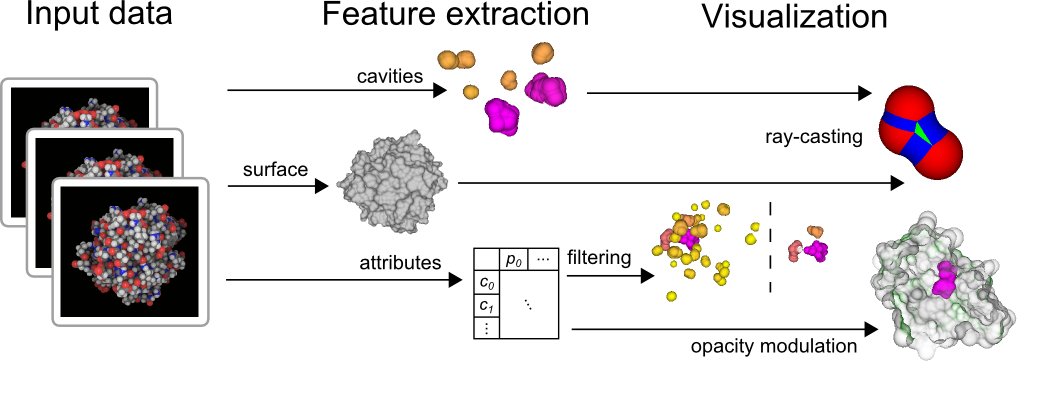
\includegraphics[width=\textwidth]{image/overview.png}
  \caption{\textcolor{red}{TODO}.}
	\label{fig:overview}
\end{figure*}

%Overview (0.5 page) (AJ, JP)
%\begin{itemize}
%  \item "Technical Part" (AJ)
%  \item SES
%  \item Cavity
%  \item Ray-casting + parameters for vis
%\end{itemize}

%\subsection{Overview}
The computation of SES is not a trivial task, which also requires a substantial computation and algorithmic capabilities. 
Therefore, it would be essential to posses a technique that could provide us with instant computation and interactive and meaningful visualization of cavities in the context of molecular surface.

The data comes in a form of MD trajectories describing the motion of individual atoms. 
Each trajectory time step includes a set of atoms, described by their positions and their radii. 
Our rendering pipeline consists of several steps that are performed on a per-frame basis. 
For better explanation, we split the computations into two groups. 
The first group deals with data processing that involves the computation of the surface primitives, and inner voids (\textcolor{red}{cavities}).
The second group of computations relates to visualization. 
This includes estimating sizes of voids, ray-casting of the formed primitives and opacity calculation; before the final stage represented by the image formation. More specifically, we perform the following steps:
	\begin{enumerate}
	  \item We employ the contour-buildup algorithm to construct the molecular surface. Additionally, we enhance the computation to enable transparent rendering of the surface and extraction of \textcolor{red}{cavities} (see Sec.~\ref{sec:ecb}).
		\item For \textcolor{red}{cavity} extraction, we introduce the so-called \textit{surface graph} (Sec.~\ref{sec:graph}), which allows us to detect isolated surface features.
		\item We estimate area of the extracted cavities to enable color coding by their size and to lower possible clutter by hiding small cavities.
		\item Surface features are visualized using ray-casting (Sec.~\ref{sec:vis}). We perform transparent surface rendering by means of an A-buffer. The actual opacity of each surface element is modulated through occurance of a void behind it.
	\end{enumerate}